\chapter{Desenvolvimento}
\thispagestyle{plain}
\label{cap:desenvolvimento}
\graphicspath{{./Cap3_Desenvolvimento/Figures/}}

\section{O algoritmo de detecção de objetos}

O algoritmo de detecção de objetos utilizado nesse estudo foi o \textit{Haar cascade object detection}, proposto por Viola e Jones em sua pesquisa \textit{Rapid Object Detection using a Boosted Cascade of Simple Features} \cite{Viola2001}, inicialmente proposto para detecção de faces, mas sendo possível ser utilizado na detecção de qualquier objeto. A biblioteca OpenCV fornece uma implementação desse algoritmo proposto para detecção de objetos \cite{OpenCV-CascadeClassifier}, que pode ser usando tanto para o treinamento de um novo modelo quanto para realizar a detecção em si, utilizando-se do modelo treinado ou de algum dos modelos pretreinados disponibilizados pelos próprios mantenedores do OpenCV em \cite{OpenCV-PreTrainedModels}. Neste trabalho foi utilizado o modelo pretreinado 'haarcascade\_frontalface\_alt.xml' para a detecção das faces. 

Não é o algoritmo com melhor acurácia atualmente, se comparado com técnicas mais modernas que aplicam \textit{deep learning}, porém é um algoritmo extremamente rápido e preciso, portanto ainda é muito útil para detecção de objetos em dispositivos com recursos limitados, como é o caso de dispositivos de borda, em geral.

Uma desvantagem nesse método é a tendência à detecção de falsos positivos. Existe também a necessidade de definição de alguns parâmetros na implementação fornecida no OpenCV, descritos resumidamente a seguir.

O método fornecido pelo objeto do tipo \emph{CascadeClassifier} \cite{OpenCV-CascadeClassifier} para performar a detecção em uma imagem é o \emph{detectMultiScale}, que tem assinatura (em C++) conforme a figura \ref{fig:detectMultiScaleFcn}. O modelo classificador pretreinado é carregado previamente utilizando-se do método \emph{load} do mesmo objeto.

\begin{figure}[h]
    \centering
    \caption[Assinatura da função detectMultiScale do OpenCV.]{Assinatura da função detectMultiScale do OpenCV.}
    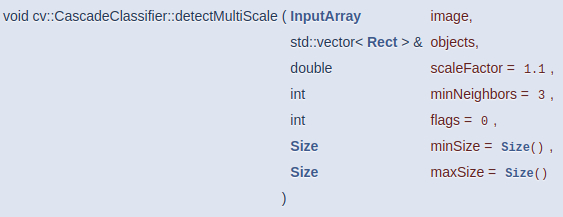
\includegraphics[width=0.60\textwidth]{Cap3_Desenvolvimento/Figures/detectMultiScaleFcn.jpg}
    \caption*{Fonte: Documentação do OpenCV.\footnotemark}
    \label{fig:detectMultiScaleFcn}
\end{figure}

\footnotetext{Disponível em: <https://docs.opencv.org/3.2.0/d1/de5/classcv\_1\_1CascadeClassifier.html>}

\begin{itemize}
    \item \emph{image} - matriz da imagem de entrada, na qual os objetos (no nosso caso, faces) serão detectados;
    \item \emph{objects} - referência ao vetor de retângulos que será populado com as áreas na imagem de entrada onde foram detectadas as faces;
    \item \emph{scaleFactor} - esse parâmetro determina o quanto a imagem será reescalonada em cada passo durante a detecção. O modelo foi treinado com imagens de tamanhos fixos, então, para possibilitar a detecção de variados tamanhos de faces, a imagem tem sua resolução reduzida em vários passos, de forma que em algum determinado passo faces maiores tenham proporções próximas da utilizada no treinamento do modelo e, assim sejam detectadas. Por exemplo, um valor de 1.1 significa que a imagem será reduzida 10\% a cada passo, um valor de 1.05, 5\%. Quanto menor for o valor desse parâmetro maiores serão as chances de uma face se encaixar ao tamanho detectável em algum passo, porém mais lento será a resposta do algoritmo já que será exigido mais processamento conforme aumenta a quantidade de passos.
    \item \emph{minNeighbors} - especifica quantos vizinhos cada retângulo candidato a uma face deve ter para ser considerado como uma detecção positiva. Em resumo, esse parâmetro afeta na qualidade da resolução. Valores baixos podem detectar maiores quantidades de faces porém com a presença de muitos falsos positivos, enquanto valores maiores tendem a aumentar a confiabilidade do que é detectado porém podendo aumentar a quantidade de falsos negativos (quando há uma face mas não é detectada pois não tem retangulos vizinhos suficientes);
    \item \emph{flags} - não utilizado;
    \item \emph{minSize} - indica o tamanho mínimo de face a ser detectada na imagem. Tamanhos mínimos maiores tendem a reduzir o tempo de resposta por aumentar o tamanho da janela deslizante na varredura da imagem (o que demanda mais processamento), mas com risco de não detectar faces relativamente pequenas. Tamanhos mínimos menores aumentam as chances de detecção de faces relativamente pequenas, mas com aumento também na demanda de processamente devido à dimuinuição da janela deslizante.
    \item 
\end{itemize}

O ajuste de parâmetros não é muito simples e depende do cenário da imagem, dos possíveis tamanhos de faces que se dejesa detectar, etc. A escolha dos parâmetros influencia diretamente no resultado da detecção, na capacidade de detecção de determinados tamanhos de faces, na propensão em detectar falsos-positivos e no tempo de execução.

Devido a isso, viu-se necessário o desenvolvimento de uma ferramenta para se testar de uma só vez um range variável de valores de determinados parâmetros e verificar facilmente a qualidade e tempo de detecção para cada combinação de valores testados. 

\section{Ferramenta de parametrização, otimização e obtenção de resultados}

O \textit{design} da ferramenta foi pensado de forma a facilitar a análise do resultado de diversas combinações de parâmetros ao mesmo tempo, de diferentes imagens e em dispositivos diferentes, através de uma interface web.

Contitui de duas partes: a parte cliente, uma interface web que pode ser executada em qualquer dispositivo através de um navegador, e a parte servidor, que deve rodar nos dispositivos que serão testados.

No cliente é feita a seleção da imagem a ser utilizada no teste, é definido o endereço do dispositivo a ser testado, rodando o servidor, e são definidos os parâmetros de testes. O cliente envia os dados para o servidor que executa o algoritmo de detecção conforme os parâmetros passados e retorna para o cliente o resultado de cada combinação de valores dos parâmetros solicitados. O resultado é composto por uma matriz contendo o tempo médio de execução, a quantidade de faces detectadas e a posição de cada face detectada para cada par de valores dos parâmetros na matriz. As faces detectadas são vizualizadas na imagem ao se selecionar um dos resultados, permitindo, assim, a verificação da qualidade da de detecção e a presença de falsos-positivos.

Na figura a seguir temos um exemplo da interface com imagem e parâmetros selecionados, ainda sem exibição do resultado da análise.

\begin{figure}[h]
    \centering
    \caption[Interface e seus parâmetros.]{Interface e seus parâmetros.}
    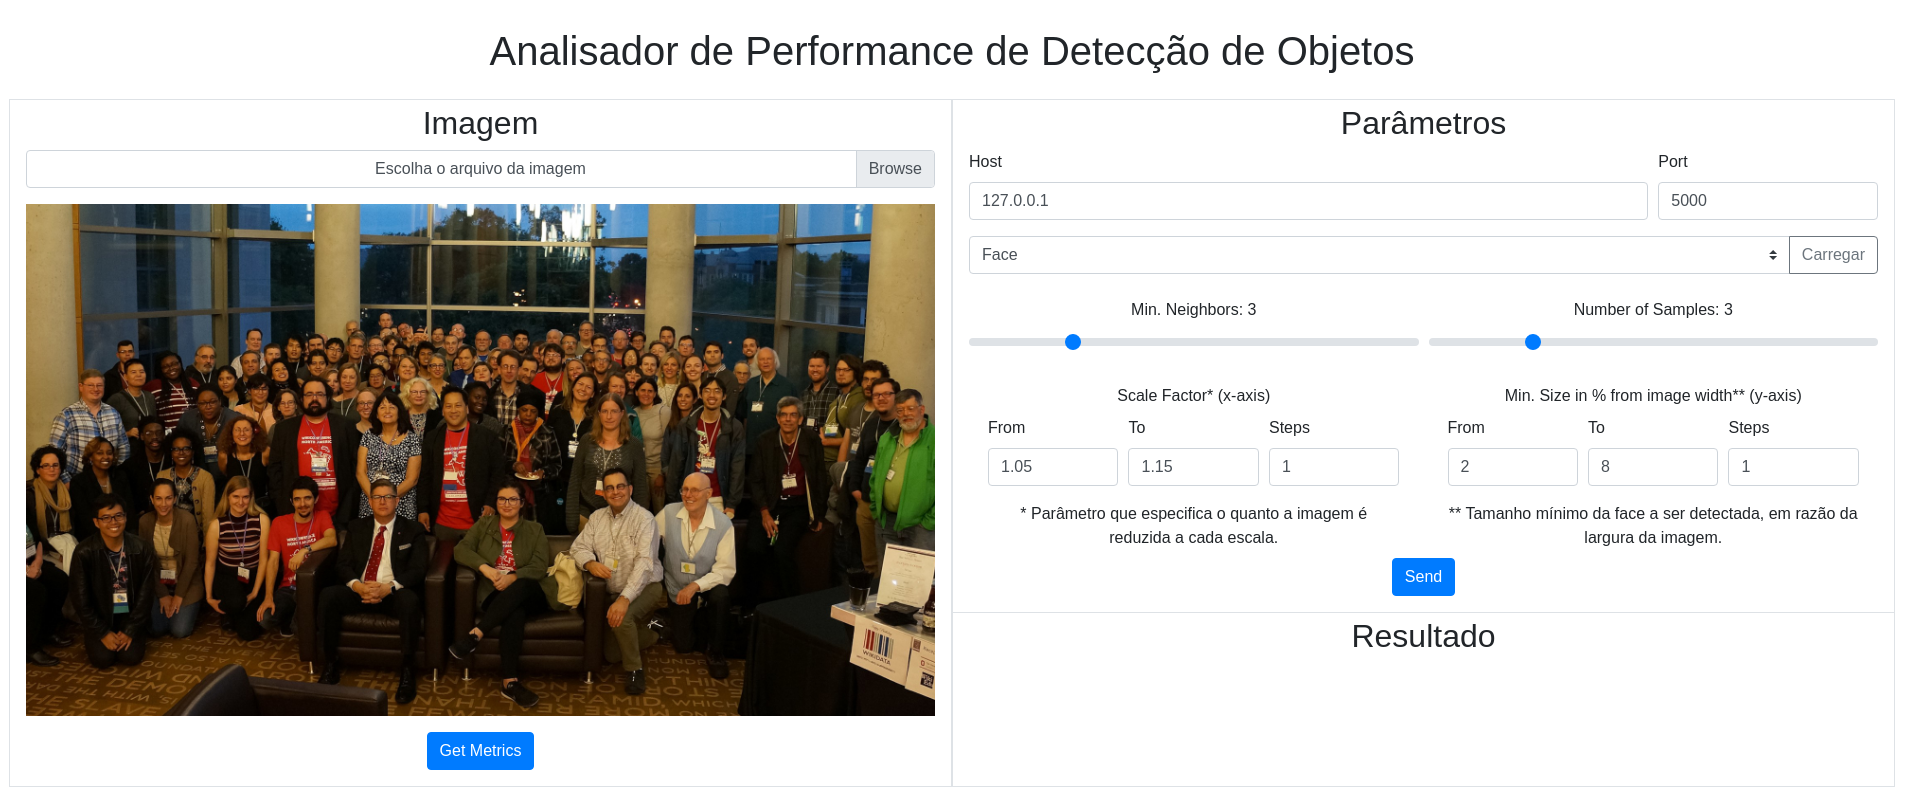
\includegraphics[width=1.0\textwidth]{Cap3_Desenvolvimento/Figures/interface_parametros.png}
    \caption*{Fonte: compilação do autor.\footnotemark}
    \label{fig:interfaceUsuario}
\end{figure}

\footnotetext{Imagem usada na compilação disponível em: <https://commons.wikimedia.org/wiki/File:WikiConference\_North\_America\_2018\_-\_Friday\_Group\_Photo.jpg>
Arquivo de imagem sob a licença CC BY-SA 4.0: <https://creativecommons.org/licenses/by-sa/4.0/deed.en>}


À esquerda da interface há um elemento de entrada que permite a seleção a imagem a ser utilizada no ensaio. Na imagem, exibida logo abaixo, serão delimitadas as faces detectadas.

À direita há dois campos, "Host" e "Port", que permitem a seleção do dispositivo a ser testado, a partir do endereço IP e porta em que a aplicação estará "escutando".

Logo abaixo estão os parâmetros a serem definidos e enviados ao servidor para a execução do ensaio. Três deles, "Scale factor", "Min neighbors" e "Min size", são parâmetros passados na própria função \textit{detectMultiScale} do OpenCV, e o significado de cada um foi descrito no início desta seção. O parâmetro "Number of Samples" determina quantas vezes o servidor executa cada combinação de parâmetros para obter um resultado médio.

Para o parâmetro "Min Neighbors", é possível definir apenas um valor para cada execução, que será utilizado em todas as combinações de parâmetros. Já para os parâmetros "Scale Factor" e "Min Size" é possível definir valores mínimos, máximos e as quantidade de valores ("Steps") a serem distribuidos linearmente nos intervalos definidos para cada um dos dois parâmetros. O servidor executará todas as combinações possíveis a partir dos conjuntos de valores delimitados, e retornará uma matriz com um resultado para cada combinação.

Por fim, ao se clicar no botão "Send", a imagem e os parâmetros são enviados para o servidor. O servidor executa o algoritmo de detecção com todas as combinações possíveis e retorna uma matriz de resultados contendo número de faces detectadas e tempo médio de execução.

\begin{figure}[h]
    \centering
    \caption[Exemplo de resultado retornado.]{Exemplo de resultado retornado.}
    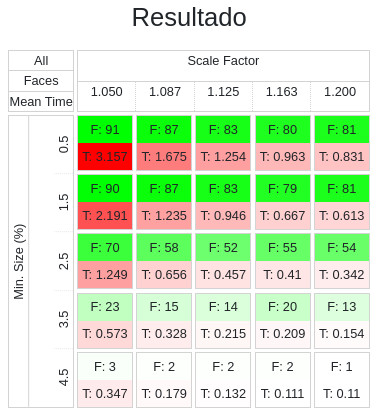
\includegraphics[width=0.6\textwidth]{Cap3_Desenvolvimento/Figures/exemplo_resultado_matriz.jpg}
    \caption*{Fonte: autor.}
    \label{fig:matrizResultado}
\end{figure}

Como pode ser visto na figura \ref{fig:matrizResultado}, o resultado é exibido em forma de uma matriz. No eixo vertical têm-se a distribuição dos valores definidos para o parâmetros "Min. Size" e no eixo horizontal têm-se a distribuição dos valores definidos para o parâmetro "Scale Factor", de conforme os limites e quantidades de passos definidos para cada um.

Cada célula da matriz apresenta o resultado da detecção, utilizando a combinação de parâmetros corresponde, com base em duas métricas, a quantidade de faces detectadas, na parte superior da célula, e o tempos médio em segundos, na parte inferior da célula. Importante ressaltar que o tempo médio refere-se ao tempo que o algoritmo levou para a detecção de todas as faces detectadas, e não ao tempo médio de execução de cada face. A média se dá de acordo com a quantidade de vezes que o algoritmo de detecção foi executado para cada combinação de parâmetros, definido em "Number of Samples".

Em uma primeira análise, a partir resultado do exemplo dado na figura \ref{fig:matrizResultado}, é possível observar a tendência de se ter maior quantidade de faces detectadas, bem como maior tempo de execução, quanto mais ao topo e à esquerda está a célula na matriz. Essa observação é um tanto óbvia tendo em vista que quanto menor o tamanho mínimo de faces a ser considerado pelo algoritmo (parâmetro "Min. Size"), mais faces candidatas tendem a ser encontradas e também mais iterações serão realizadas. O mesmo acontece para o parâmetro "Scale Factor", quanto menor o valor do parâmetro, menor o passo entre as escalas, maior a quantidade de imagens escalonadas avaliadas e, portanto, maior a chance de de uma determinada face ser detectada, bem como maior quantidade de iterações realizadas.

A matriz de resultados por si só não é suficiente para se determinar que uma combinação de parâmetros é a mais adequada a se adotar. Isso se deve ao fato de que não se pode afirmar que o resultado com o maior número de faces detectadas é o melhor pois, dentro do conjunto de faces detectadas, alguma poucas ou até várias delas podem ser falsos positivos, de tal forma que a qualidade do resultado da detecção deva ser considerado ruim. 

Outra questão a se considerar é que, dependendo do ambiente e do objetivo da aplicação, a detecção da maior quantidade de faces possível pode não ser a prioridade. Em determinado tipo de aplicação, pode ser mais interessante que o algoritmo detecte apenas faces que estejam mais próximas da câmera (e por conta disso relativamente maiores que as demais), com um tempo de resposta menor, do que detectar o máximo de faces possível, inclusive as mais distantes, que seriam descartadas, com um tempo de resposta maior.

Para tanto, é importante que haja uma análise qualitativa, ao se checar, para cada resultado analisado, quais foram as faces detectadas, resultantes da correspondente combinação de parâmetros. E, a partir da avaliação dos resultados disponíveis, comparando a presença de falsos positivos, a quantidade e tamanho das faces detectadas e o tempo médio de resposta, determinar uma combinação de parâmetros mais adequada a se adotar em uma aplicação de detecção no dispositivo testado ou concluir que o dispositivo não seria capaz de rodas a aplicação da forma desejada.

Para facilitar esse tipo de análise qualitativa, a matriz de resultados responde de forma interativa, de forma que, ao se clicar em uma célula da matriz, as faces detectadas a partir dos parâmetros correspondentes daquela célula são destacadas na imagem original através de retângulos verdes, facilitando assim a verificação de falsos positivos e quais faces presentes na imagem o algoritmo conseguiu detectar com tais parâmetros.

A seguir são apresentados alguns exemplos de resultados, a partir da matriz de resultado apresentada na figura \ref{fig:matrizResultado}. Para facilitar a visualização, serão apresentados apenas os cortes da matriz com o resultado selecionado e a imagem com as faces destacadas.

No exemplo da figura \ref{fig:exemploResultado1}, têm-se um resultado com muito poucas faces detectadas devido ao valor relativamente alto do parâmetro "Min. Size".

Já a figura \ref{fig:exemploResultado2} apresenta um resultado com várias faces detectadas, inclusive pequenas faces ao fundo. Porém, devido aos valores relativamente baixos dos parâmetros "Min. Size" e "Scale Factor", vê-se claramente a presença de três falsos positivos, além de um tempo médio de detecção consideravelmente alto, acima de 3 segundos.

Por fim, a figura \ref{fig:exemploResultado3} apresenta um resultado que possivelmente pode ser considerado satisfatório para determinados tipos de aplicação. Nesse caso, a maioria das faces presentes na imagem foi detectada e com um tempo de resposta razoavelmente baixo, pelo menos se comparado ao resultado apresentado na figura \ref{fig:exemploResultado2}.

\begin{figure}[h]
    \centering
    \caption[Exemplo de resultado com poucas faces detectadas.]{Exemplo de resultado com poucas faces detectadas.}
    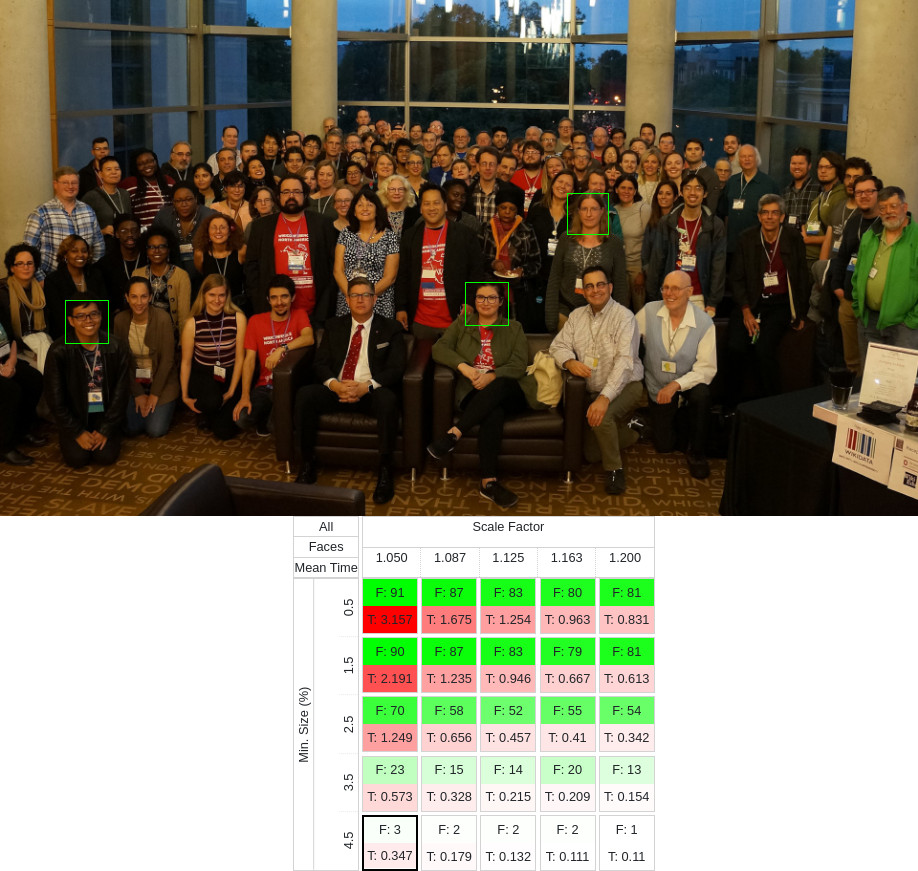
\includegraphics[width=0.8\textwidth]{Cap3_Desenvolvimento/Figures/exemplo_resultado_1.jpg}
    \caption*{Fonte: compilação do autor.\footnotemark[\value{footnote}]}
    \label{fig:exemploResultado1}
\end{figure}

\begin{figure}[h]
    \centering
    \caption[Exemplo de resultado com várias faces detectadas e alguns falsos positivos.]{Exemplo de resultado com várias faces detectadas e alguns falsos positivos.}
    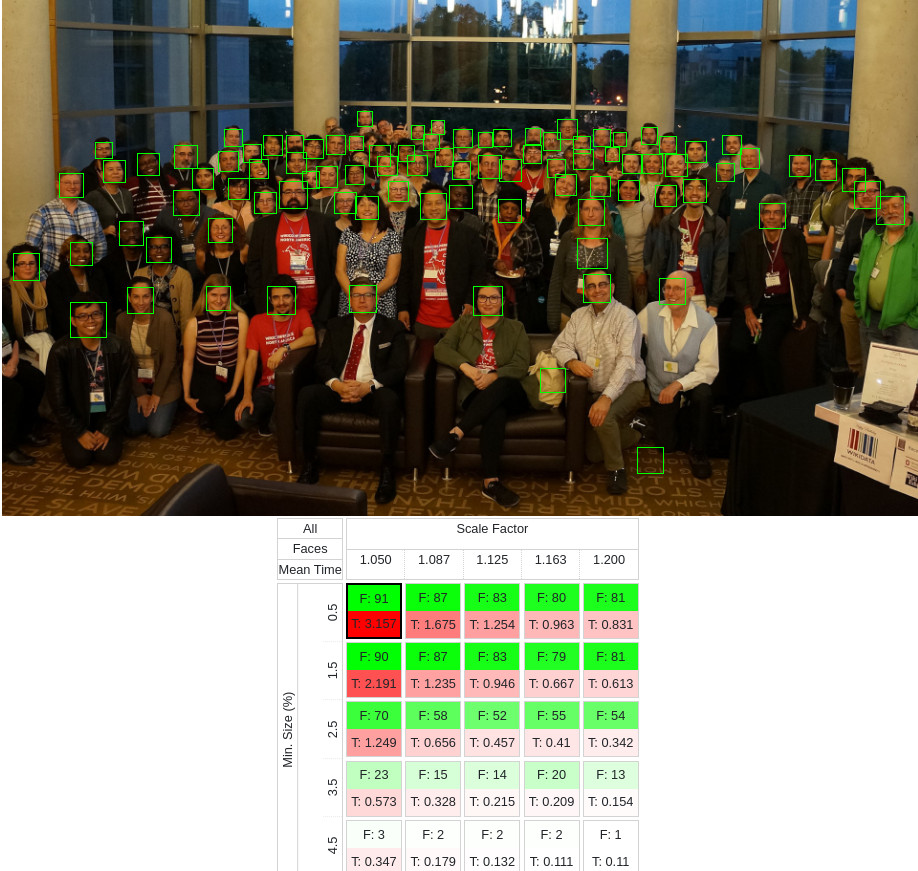
\includegraphics[width=0.8\textwidth]{Cap3_Desenvolvimento/Figures/exemplo_resultado_2.jpg}
    \caption*{Fonte: compilação do autor.\footnotemark[\value{footnote}]}
    \label{fig:exemploResultado2}
\end{figure}

\begin{figure}[h]
    \centering
    \caption[Exemplo de resultado possivelmente satisfatório.]{Exemplo de resultado possivelmente satisfatório.}
    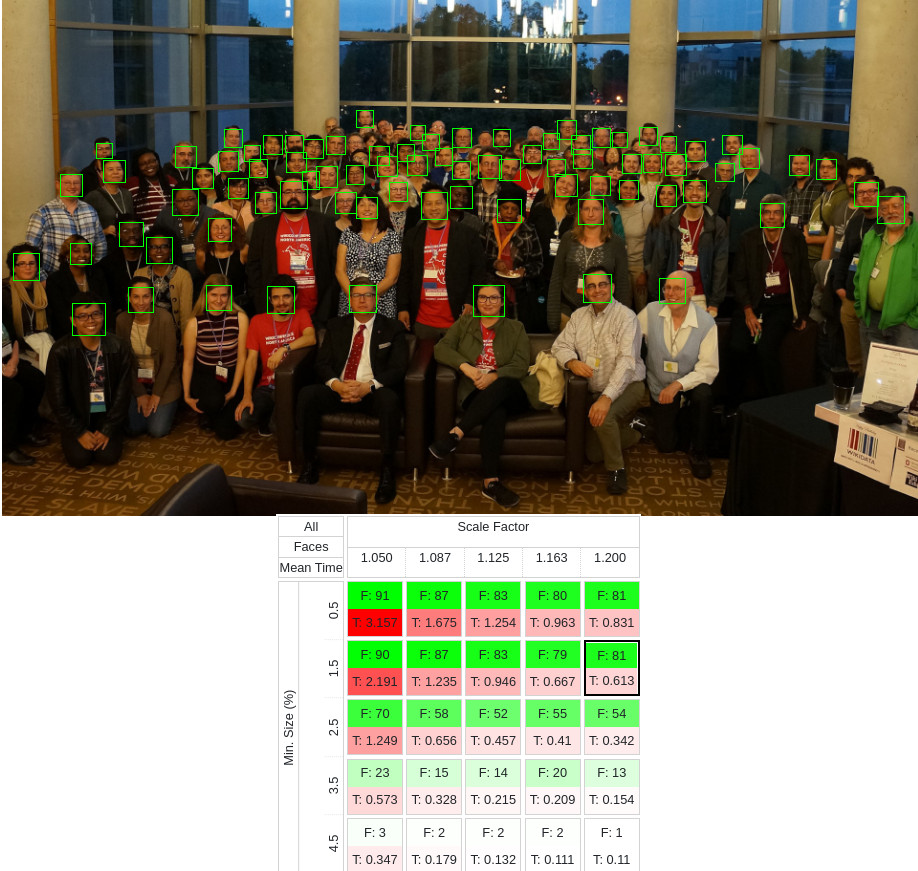
\includegraphics[width=0.8\textwidth]{Cap3_Desenvolvimento/Figures/exemplo_resultado_3.jpg}
    \caption*{Fonte: compilação do autor.\footnotemark[\value{footnote}]}
    \label{fig:exemploResultado3}
\end{figure}


Outra facilidade que a ferramenta traz é quanto à flexibilidade na escolha dos limites e quantidades de valores a serem testados para cada parâmetros, permitindo, assim, ajustar os mesmos iterativamente, de forma a se ter cada vez melhores resultados e, consequentemente, melhores opções de otimização.

Ainda partindo da matriz de resultados da figura \ref{fig:matrizResultado}, alguns limites podem ser ajustados para uma próxima rodada de análise. Por exemplo, observa-se que nos resultados em que o valor de "Min. Size" é maior que 2.5, a quantidade de faces detectadas é muito baixa. Caso seja considerado insatisfatório, o novo valor máximo na distribuição desse parâmetro pode ser definido como 2.5 ou 3.0. Analisando o parâmetro "Scale Factor", pode-se observar que valores abaixo de 1.125 resultam em um tempo de resposta muito alto e apresenta muitos falsos positivos. Além disso, alguns resultados com o valor máximo apresentado de "Sacle Factor", 1.200, apresentam uma quantidade alta de faces detectadas, sendo possível que um valor maior possa apresentar um resultado igualmente bom mas com um tempo de resposta menor. Os limites de "Scale Factor" poderiam ser ajustados, por exemplo, para 1.080 e 1.250. Assim, uma próxima rodada de análise com os limites ajustados irão retornar uma maior e melhor gama de resultados.

A título de exemplo, a figura \ref{fig:matrizResultado2} apresenta a matriz de resultado com os limites ajustados. Observa-se uma melhor distribuição, com números de faces detectadas e tempo de resposta mais próximos do que podem ser considerados como satisfatórios, possibilitando uma análise mais precisa para determinar os melhores parâmetros.

\begin{figure}[h]
    \centering
    \caption[Exemplo de matriz de resultado com limites ajustados.]{Exemplo de matriz de resultado com limites ajustados.}
    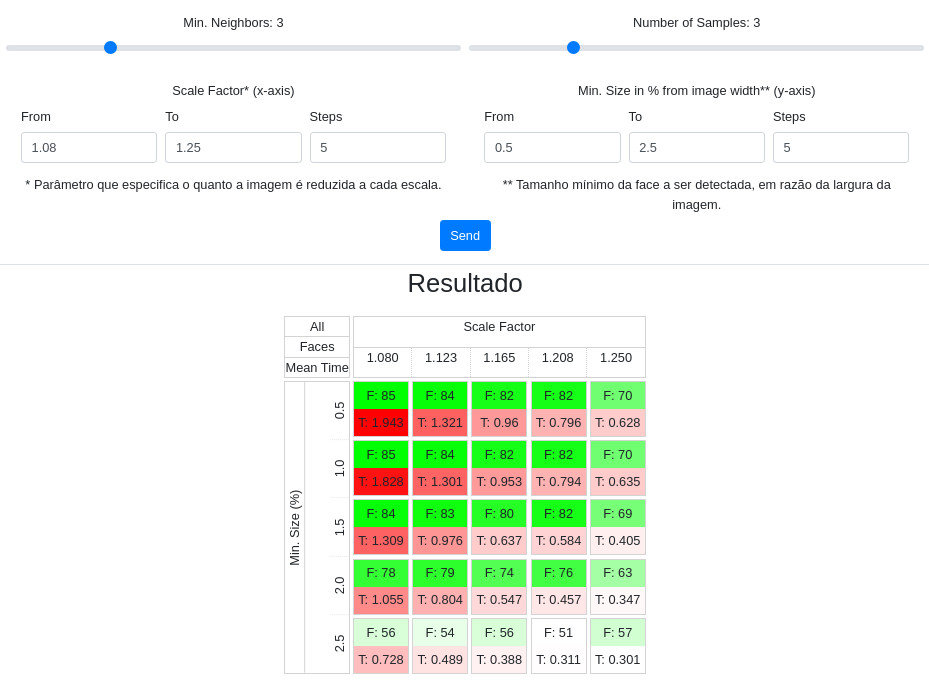
\includegraphics[width=0.8\textwidth]{Cap3_Desenvolvimento/Figures/exemplo_resultado_matriz_2.jpg}
    \caption*{Fonte: autor.}
    \label{fig:matrizResultado2}
\end{figure}

Há de se observar que, pelo fato de a análise estar sendo feita a partir de apenas uma imagem, não é de se esperar que o resultado quanto à presença, ou não, de falsos positivos, seja o mesmo para todos os frames que serão analisados em uma aplicaćão real, mesmo a câmera estando fixa, capturando sempre o mesmo cenário.

Em uma aplicação real da ferramenta, é interessante que os valores escolhidos dos parâmetros sejam testados utilizando-se outras imagens da mesma cena com suas possíveis variações, como por exemplo a diferente quantidade de pessoas e objetos, iluminações diferentes, etc.

Tendo definido-se uma melhor combinação de valores dos parâmetros, pode-se então obter uma análise mais aprofundada, com métricas adicionais, que auxiliará na análise e comparação dos resultados entre os diferentes cenários e dispositivos testados. Os resultados serão analisados considerando não só qualidade de deteção e tempo de reposta, como também a demanda de banda em rede e quantidade de dados trafegados para se progragar o resultado a uma próxima etapa de processamento dentro de um sistema distribuído.

Ao se clicar no botão "Get Metrics", no lado esquerdo da tela (vide figura \ref{fig:interfaceUsuario}), os parâmetros definidos de acordo com a célula selecionada na matriz de resultados são enviados ao servidor no dispositivo que está sendo testado. Este, por sua vez, executa novamente o algoritmo de detecção, logando também o tempo de execução de outras etapas preparatórias, bem como outras informações referentes aos tamanhos das imagens.

Na figura \ref{fig:resultadoMetricas}, pode-se observar como os dados retornados são exibidos na interface do usuário. A seguir, uma breve explicação de cada item:

\begin{itemize}
    \item 1.0 - Params: os parâmetros utilizados no algoritmos de detecção, conforme célula selecionada na matriz de resultados na etapa anterior;
    \item 1.1 - Full Image Resolution: a resolução da imagem original, em pixels;
    \item 1.2 - Full Image Size (bytes): o tamanho da imagem original, em bytes;
    \item 1.3 - Full Image Encoded Size (bytes): o tamanho da imagem original codificada em bitmap e base64, em bytes;
    \item 1.4 - Number of detected faces: o número de faces detectadas;
    \item 1.5 - Cropped Faces Images Total Size (bytes) / (\% from full image size): o tamanho total das imagens de faces detectadas, recortadas da imagem original, em bytes, e o seu percentual com relaçãao ao tamanho da imagem original;
    \item 1.6 - Encoded Faces Images Total Size (bytes) / (\% from full image size): o tamanho total das imagens de faces detectadas, codificadas em bitmap e base64, em bytes, e o seu percentual com relação ao tamanho da imagem original codificada;
    \item 2.1 - Loading Image (s): o tempo de carregamento da imagem original (leitura em disco), em segundos;
    \item 2.2 - Convert Image to Gray (s): o tempo de conversão da imagem original para escala de cinza, em segundos. Etapa anterior necessária para execução do algoritmo de detecção;
    \item 2.3 - Detection (s): o tempo de execução do algoritmo de detecção em si, em segundos;
    \item 2.4 - Build Encoded Faces Images (s): o tempo de execução da etapa de encodamento das imagens em base64, em segundos;
    \item 2.5 - Total execution time (s): o tempo total de execução e todas as etapas, desde o carregamento da imagem até o encodamento em base64, em segundos.
    \item 3.1 - Faces images: as imagens das daces detectadas, recortadas da imagem original em seu tamanho real. Permite se ter uma ideia da qualidade de resolução individual das faces, bem como facilita a identificar mais facilmente a presença de falsos positivos que possam não terem sido identificados na etapa de análise anterior.
\end{itemize}

\begin{figure}[h]
    \centering
    \caption[Exemplo de resultado com as métricas.]{Exemplo de resultado com as métricas.}
    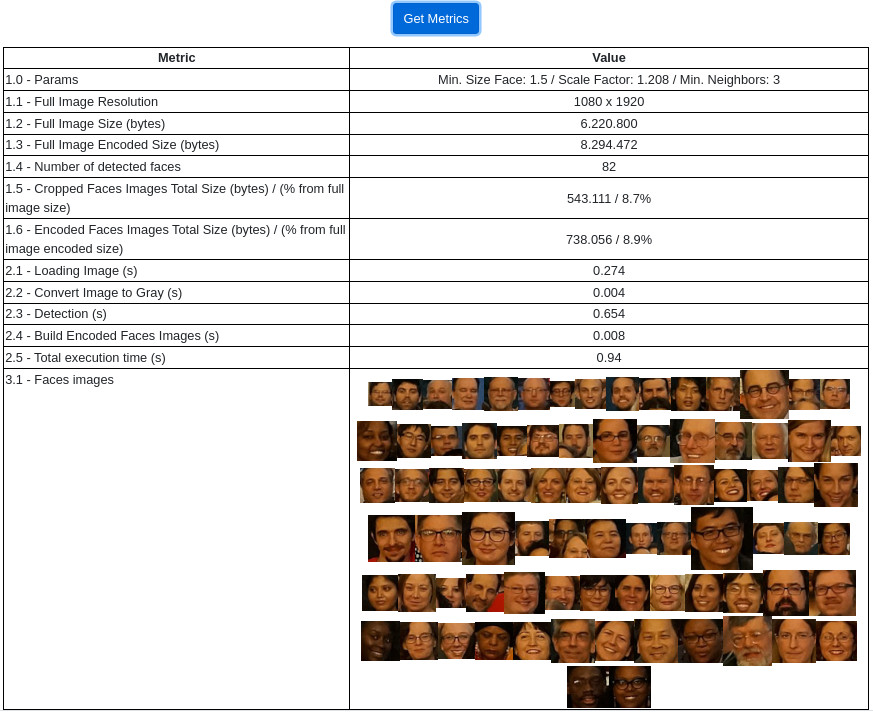
\includegraphics[width=0.8\textwidth]{Cap3_Desenvolvimento/Figures/exemplo_metricas.jpg}
    \caption*{Fonte: autor.}
    \label{fig:resultadoMetricas}
\end{figure}

É importante ressaltar que, como os testes são feitos a partir de imagens pré-selecionadas, a métrica 2.1 considera o tempo de carregamento em memória da imagem salva em disco. O problema é que esse tempo é limitado apenas pela velocidade de leitura no sistema de arquivos, enquanto que em uma aplicação real a aquisição das imagens se darão a partir de uma fonte, como um sensor conectado à placa, uma câmera USB ou via streamming, por exemplo.

Para se ter no estudo um tempo de aquisição de imagem mais realista, foram feitos testes à parte para se obter o tempo médio de captura a partir de um módulo de câmera conectado diretamente ao dispositivo. Foi utilizado um módulo com sensor OmniVision OV5647, com capacidade de capturar imagens com resolução de até 2592x1944, e interface CSI, próprio para ser utilizado com um Raspberry Pi. Para captura de imagens, foi utilizado o pacote \emph{picamera}, que provê uma interface simplificada em Python para o módulo da câmera.

Segundo a própria documentação \cite{Picamera}, o pacote \emph{Picamera} oferece diferentes formas de se fazer a captura de imagens, chamados de \emph{ports}. De acordo com o \emph{port} utilizado, a câmera se comporta de maneira diferente durante a captura, o que irá influenciar na qualidade da imagem e tempo de aquisição dos frames. Como cada cena possui uma proposta diferente de aplicação, os testes de tempo médio de captura foram feitos de forma diferentes e mais adequada a cada cena e serão melhores detalhados nas póximas subseções da seção a seguir.

\section{Cenários de testes}

Nesta seção são apresentados os dois cenários definidos para os testes. Cada cenário representa uma possível aplicação diferente e possui diferentes requisitos que servirão de balizas para a calibração e comparação dos resultados.

Para um estudo mais completo, serão testadas algumas variações de cada cenário, seja quanto à quantidade de faces presentes e/ou quanto à resolução da imagem testada, além, claro dos diferentes dispositivos que serão testados.

\subsection{Cena 1}

Nessa primeira cena deseja-se representar o monitoramento de um espaço aberto e amplo, onde é esperado um fluxo alto de pessoas e que estas possam estar a qualquer distância da câmera, sendo desejável que o dispositivo consiga detectar faces muito pequenas a ponto de maximar quantidade de faces detectadas.

\begin{itemize}
    \item \textbf{Variações possíveis} - variação de quantidade de faces e variação de resolução da imagem.
    \item \textbf{Requisitos mínimos} (para balizar a parametrização) - máximo 5 segundos de resposta.
    \item \textbf{Imagem para testes} - para representar esta cena, foi selecionada uma imagem (figura \ref{fig:imagemCena1}) com várias faces olhando na direção da câmera e em diferentes distâncias. Ter todas as faces olhando para a mesma direção, distancia-se de um cenário real, mas torna-se ideal para o estudo pois serve como um pior caso para a cena e facilita a obtenção de variações por quantidade de faces.
\end{itemize}

\begin{figure}[H]
    \centering
    \caption[Imagem selecionada para testes da cena 1.]{Imagem selecionada para testes da cena 1.}
    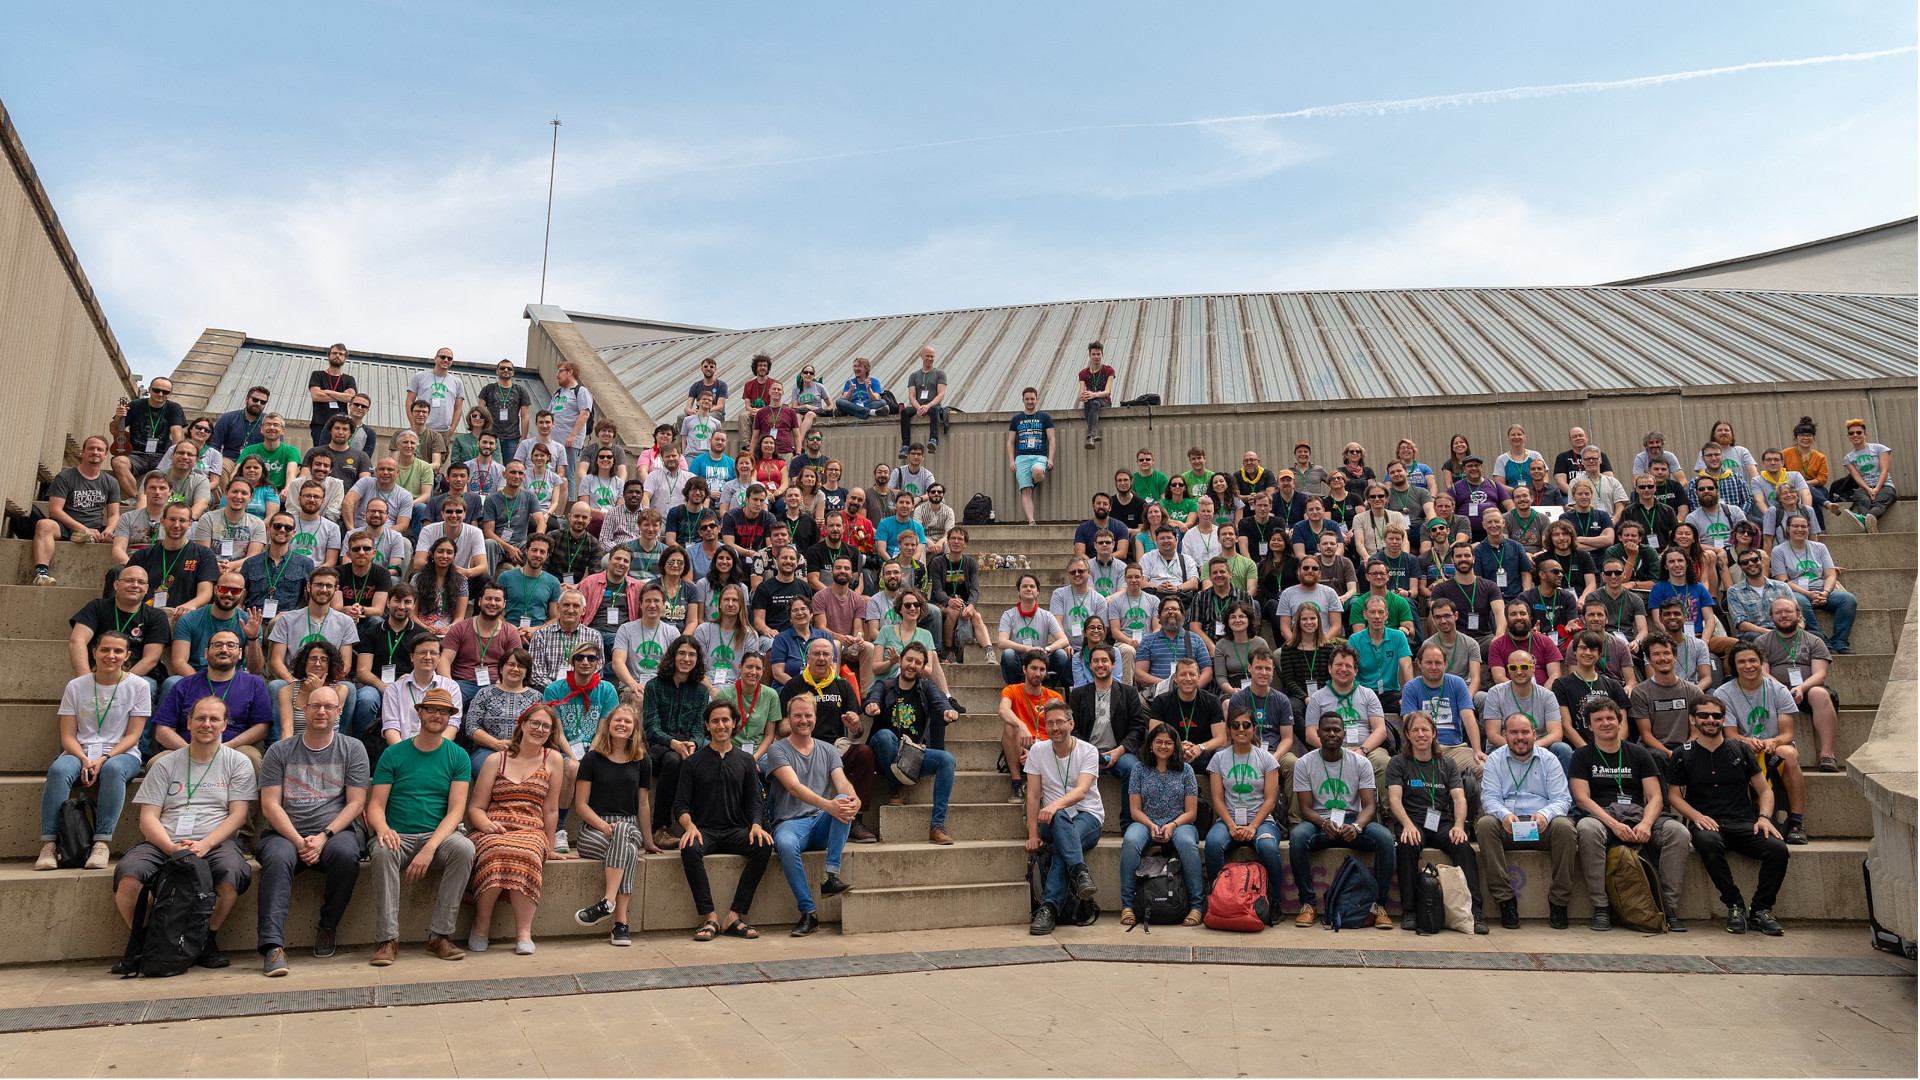
\includegraphics[width=0.8\textwidth]{Cap3_Desenvolvimento/Figures/imagem_cena1.jpg}
    \caption*{Fonte: Wikimedia Hackathon Barcelona 2018, por Ckoerner, 2018\footnotemark.}
    \label{fig:imagemCena1}
\end{figure}

\footnotetext{Disponível em: <https://commons.wikimedia.org/wiki/File:Wikimedia\_Hackathon\_Barcelona\_2018\_-\_group\_photo.jpg>
Arquivo de imagem sob a licença CC BY-SA 4.0: <https://creativecommons.org/licenses/by-sa/4.0/deed.en>}


\subsubsection{Variação de quantidade de faces}

Nessa cena, como a aplicação tem por objetivo detectar um elevado número de faces simultaneamente, pretende-se verificar como a variação da quantidade de faces presente na imagem afeta tanto no tempo de resposta do processo de detecção quanto no tamanho do conjunto das imagens das faces detectadas, recortadas da imagem completa, representando economia na utilização de banda para transmissão do resultado da detecção.

Para a realização desses testes, a escolha de uma imagem com um grande número de faces foi importante para que se pudesse obter 5 variações da mesma, reduzindo iterativamente a quantidade de faces em cada uma, da forma mais linear possível.

As variações foram preparadas utilizando-se o software de edição de imagem GIMP (GNU Image Manipulation Program), aberto e gratuito. Partindo-se da imagem original, uma certa quantidade de faces foram borradas de forma a se tornarem indetectáveis, como se aquela faces não estivessem presentes na imagem. A imagem resultante se tornou a primeira variação por quantidade de faces. A partir da imagem dessa primeira variação, foi feito o mesmo procedimento, borrando a mesma quantidade de faces que ainda não haviam sido borradas. E assim foi feito sucessivamente até obter-se um total de 5 variações. Importante ressaltar que, durante a preparação das imagens, preocupou-se em borrar as faces de uma forma bem distribuída.

\begin{figure}[h]
    \centering
    \caption[Exemplo de variação de cena com redução de 40 faces.]{Exemplo de variação de cena com redução de 40 faces.}
    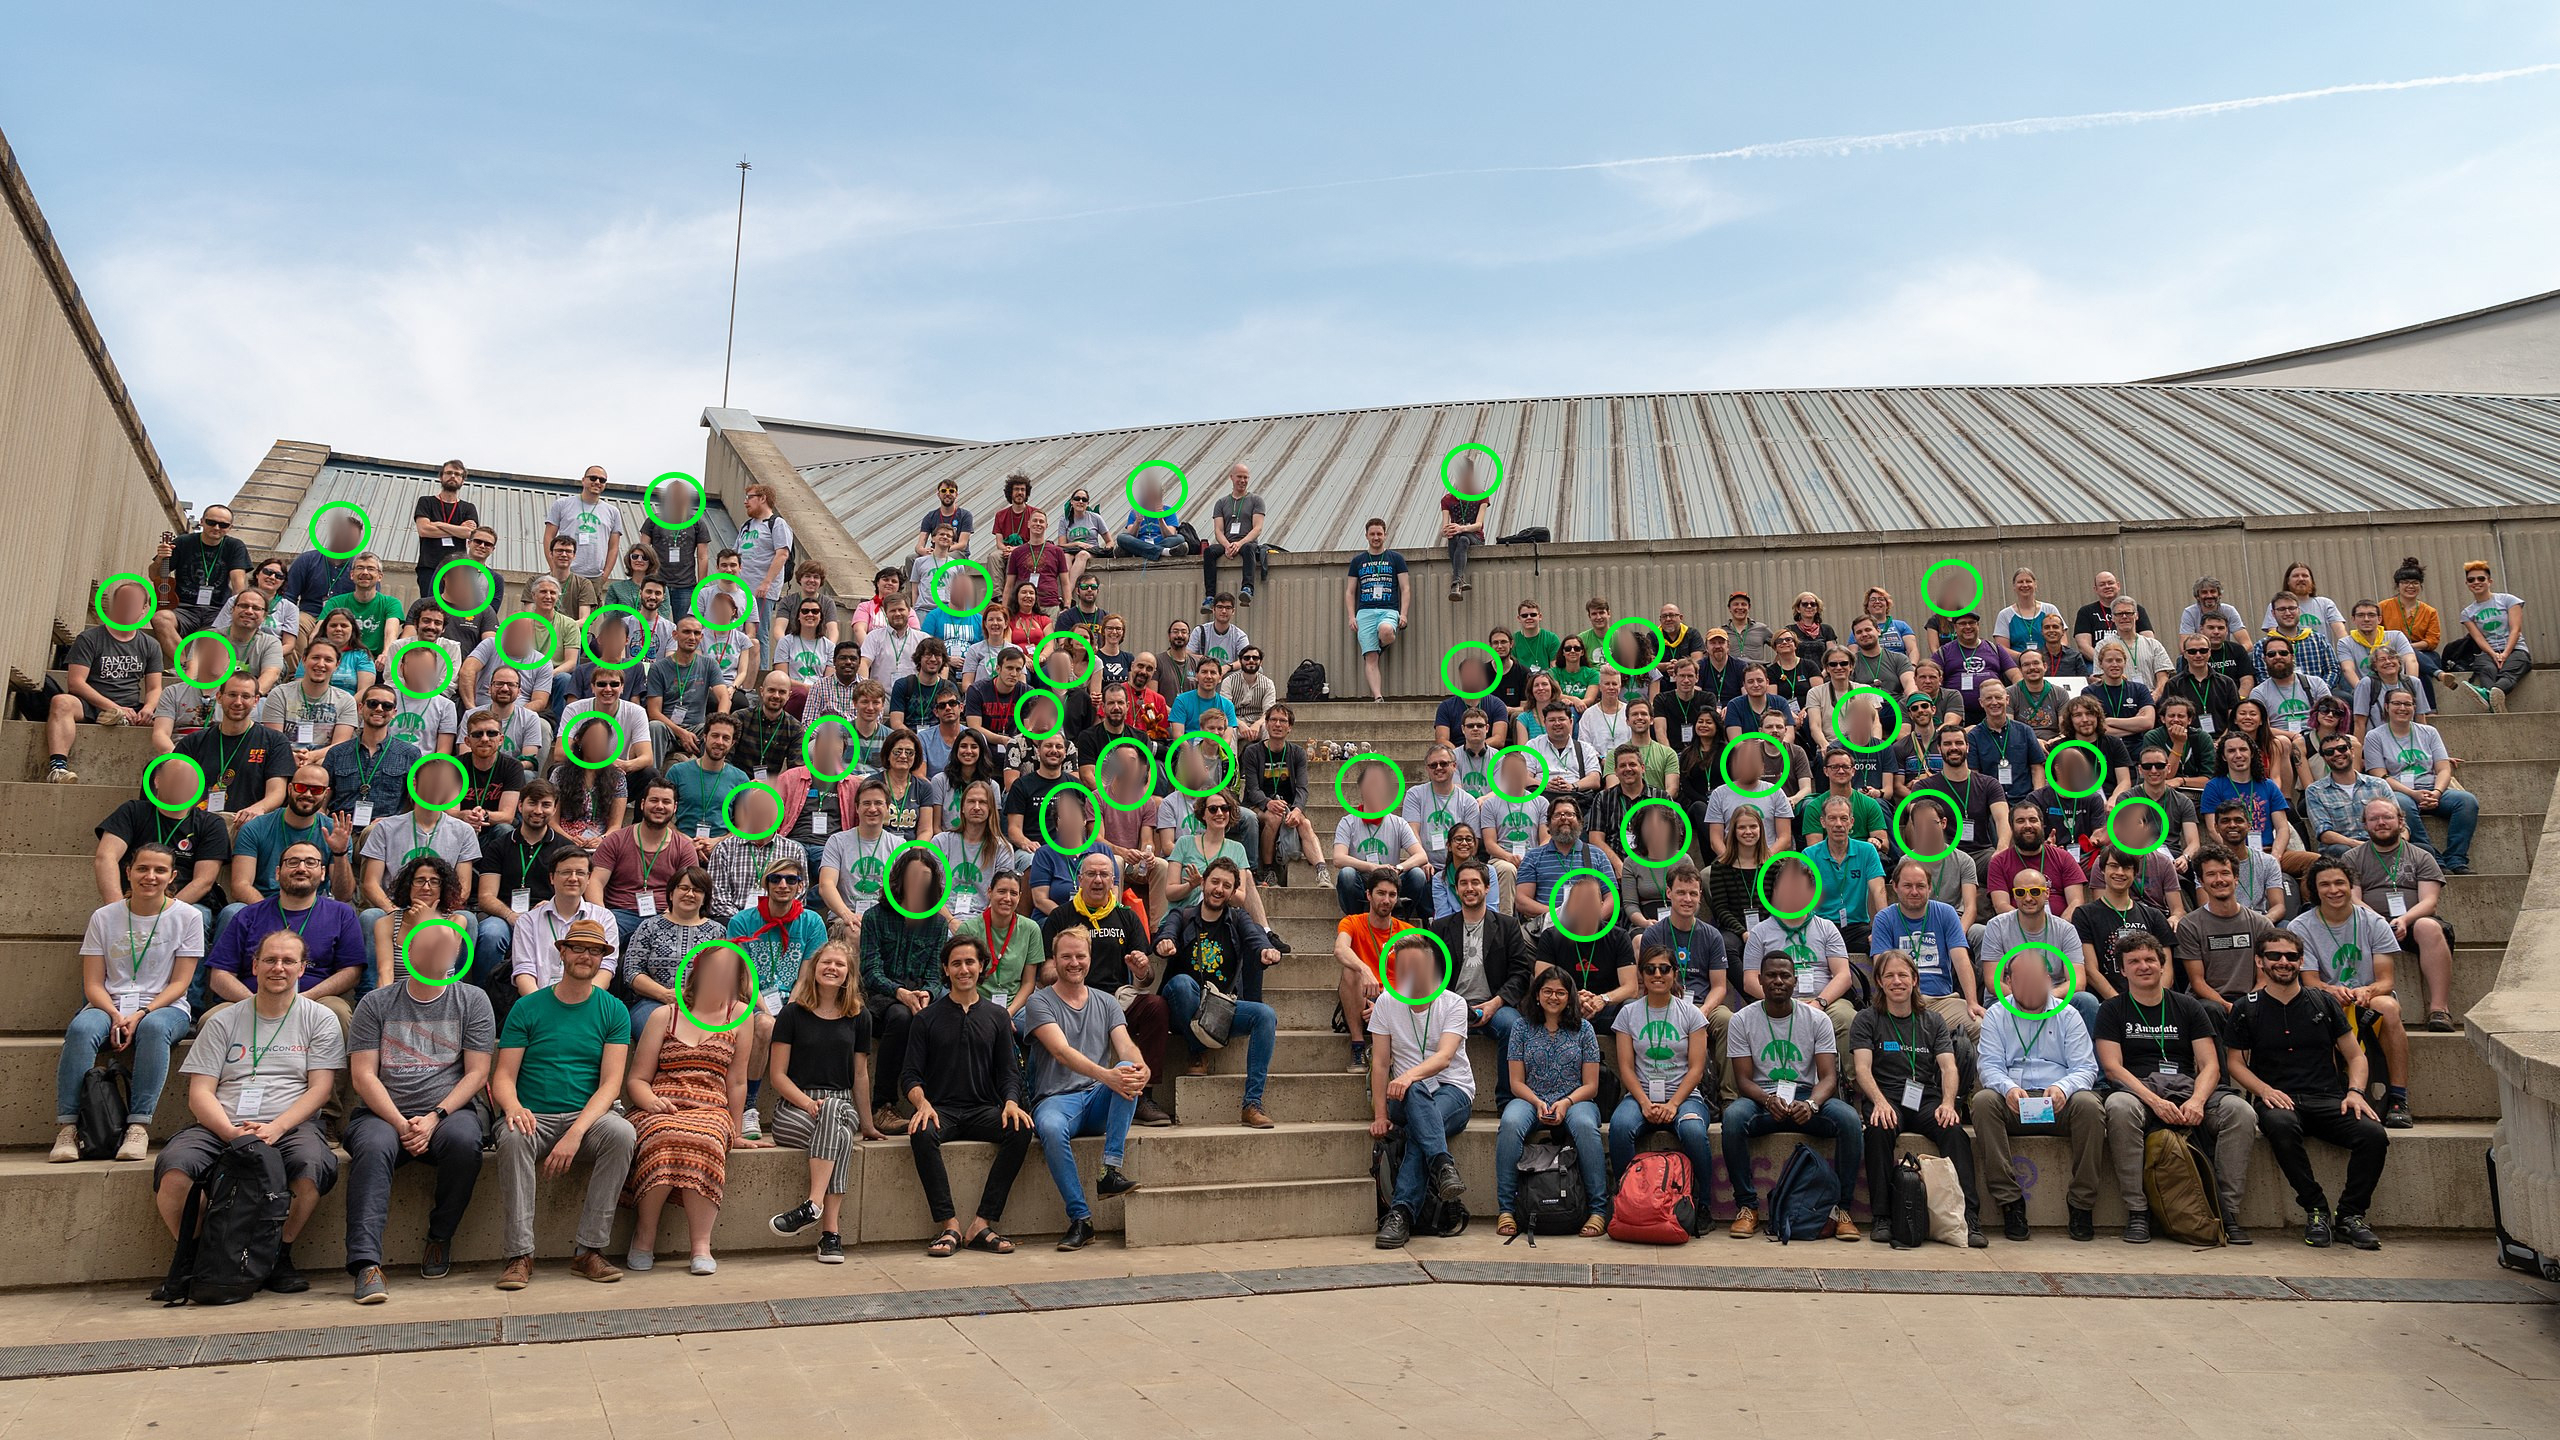
\includegraphics[width=0.9\textwidth]{Cap3_Desenvolvimento/Figures/exemplo_variacao_faces.jpg}
    \caption*{Fonte: compilação do autor.\footnotemark[\value{footnote}]}
    \label{fig:exemploVariacaoFaces}
\end{figure}

Na figura \ref{fig:exemploVariacaoFaces}, um exemplo de variação com a redução de 40 faces. Ao se comparar o resultado das variações, é de se esperar que a diferença de faces detectadas seja igual à diferente da quantidade de faces borradas, porém, não necessariamente será igual, pois pode ser que alguma face não seja detectada pelo algoritmo de qualquer forma.

Para obtenção dos dados nos testes de variação de quantidade de faces deve-se, a partir da imagem original, com todas as faces detectáveis, utilizar a ferramenta para encontrar uma combinação otimizada de parâmetros de detecção. Com os melhores parâmetros definidos, obtém-se as métricas da imagem original e também de todas a variações de quantidade de faces geradas a partir dessa mesma imagem para futura comparação.

\subsubsection{Variação de resolução da imagem}

Outra variação que é possível obter dessa mesma imagem e que fará parte do estudo é no que tange à resolução da imagem. Quanto maior a resolução da imagem, maior tende a ser a capacidade e qualidade de detecção de faces menores, mas também maior é a demanda de processamento e maior tende a ser o tempo de espera de uma detecção, bem como a utilização de banda para passar adiante as imagens das faces detectadas.

Dependendo do cenário e dos possíveis tipos de aplicação, considerar trabalhar a detecção em imagens com resoluções menores que a capacidde do sensor pode ser suficiente para viabilizar o uso do dispositivo de borda para a tarefa de detecção, desde que cumprindo os requisitos de tempo de resposta e capacidade de detecção.

Para a realização dos testes com variação de resolução, foram obtidas das imagens originais (a original e suas respectivas variações por quantidade de faces) imagens com resoluçoes menores, através de interpolação, utilizando-se também o software GIMP para o processamento. A imagem original desta cada cena foi selecionada já com resolução em quad-hd (2560x1440), e foram obtidas as variações nas resoluções full-hd (1920x1080) e hd (1280x720). Para cada redução de resolução, são obtidas 5 novas imagens, uma a partir da imagem original e outras quatro a partir da variações de quantidade de faces.

Para a obtenção dos dados nos testes de variação de resolução, utilizou-se novamente a ferramenta para encontrar a melhor combinação de parâmetros de detecção para as imagens na nova resolução e, a partir desses novos parâmetros, obteve-se as métricas de todas as imagens com a referida resolução.

\subsubsection{Tempo médio de captura}
Como já adiantado no final da seção anterior, o tempo de aquisição da imagem que será considerado no estudo será o tempo médio de captura de frames a partir de um sensor OV5647, utilizando-se o pacote \emph{Picamera}. Para a cena em questão, onde objetiva-se maximizar a quantidade de faces detectadas, podendo estas estarem bem distantes da câmera, a qualidade da imagem é um fator importante.

Um dos possíveis \emph{ports} usados pelo Picamera é o \emph{still port}, que força a captura da imagem utilizando-se toda a área do sensor, que no caso é de 2592x1944 pixels, mesmo que a resolução de saída da imagem seja menor. Além disso, usa um forte algoritmo para redução de ruído, proporcionando maior qualidade de imagem, sendo assim a forma mais adequada de considerar na captura de imagem no contexto dessa cena.

Para se obter o tempo médio de captura foi escrito um algoritmo simples, que faz a captura consecutiva de 10 frames utilizando-se o \emph{still port} e retorna o tempo médio de captura. No algoritmo é configurado a resolução de saída dos frames para corresponder às resoluções testadas.

\subsection{Cena 2}

Nessa segunda cena, deseja-se representar o controle de acesso a um ambiente, onde o dispositivo com a câmera está posicionado estrategicamente próximo à abertura de acesso (porta, portão, etc) de forma a capturar de perto a face de quem estiver adentrando ao local. É importante uma reposta rápida na detecção pois a pessoa entrando no ambiente estará em movimento, permanecendo no campo de visão da câmera por pouco tempo.

\begin{itemize}
    \item \textbf{Variações possíveis} - variação de resolução da imagem.
    \item \textbf{Requisitos mínimos} (para balizar a parametrização) - máximo 0.3 segundo de resposta com detecção a partir de 1s de distância.
    \item \textbf{Imagens para testes} - para representar esta cena, foram obtidos imagens a partir do sensor OV5647 conectado ao dispositivo, com o próprio autor simulando a entrada no ambiente.
\end{itemize}

\subsubsection{Captura das imagens para teste}

Para a captura dos frames para os testes, o dispositivo com a câmera foi posicionado estrategicamente ao lado de uma porta, a uma altura aproximada de 1,70, e levemente inclinado em direção à entrada, de forma que a câmera pudesse captar faces mais próximas e também a distâncias de até 2m.

Foram feitos testes para obter a posição de uma pessoa mais próxima da entrada em que a câmera conseguisse capturar uma boa imagem do rosto. A partir dessa posição, mediu-se 1,6 m de distância, e capturou-se novos frames, com a pessoa posicionada a essa distâcia. A partir de uma distância de aproximadamente 1,7m uma pessoa caminhando rapidamente a no máximo 6 km/h, leva pelo menos 1s para chegar à posição inicial obtida (6 km/h * 1000 m/km * 1h/3600s = 1,67m/s). A uma presença com duração de pelos menos 1s diante da câmera, com a face capturável, e a um tempo máximo de 0.3s de resposta definido na detecção, têm-se pelo menos 3 frames capturados e analizados enquando uma mesma pessoa caminha até a entrada do ambiente. Esse será considerado nosso pior caso e ambos os frames obtidos (tanto o com a pessoa na posição mais próxima da câmera quanto o com a pessoa posicionada a 1.7m da posição inicial) serão utilizados nos testes para definição dos parâmetros e obtenção das métricas para comparação.

Dessa forma, a ferramenta de análise será utilizada nessa cena com uma abordagem diferente para se obter os melhores parâmetros para comparação. Ao invés de se buscar a maior quantidade de faces detectadas no menor tempo, como feito na primeira cena, dessa vez, como o objetivo é a detecção de apenas uma face próxima por vez, busca-se encontrar os parâmetros com os quais é possível detectar a face de uma pessoa se aproximando da entrada a partir de 1,7m de distância, no menor tempo. Como têm-se duas imagens diferentes sendo analisadas, com a face da mesma pessoa, mas em posição e tamanhos relativos diferentes, cada uma apresentará resultados diferentes entre si. Portanto, serão considerados a combinação de parâmetros que atenda bem às duas imagens. Quanto aos dados obtidos das métricas para comparação de resultados, serão considerados os tempos de maior duração e os maiores tamanhos de face.

\subsubsection{Variação de resolução da imagem}

Como nessa cena considera-se a detecção de apenas uma face, variações por quantidade de faces não faz sentido. Portando, será experimentado apenas variação por resolução de imagem. 

Para a realização dos testes com variação de resolução, foram obtidas das duas imagens capturadas imagens com resoluçoes menores, através de interpolação, utilizando-se também o software GIMP para o processamento. As imagens originais originais foram capturadas já com a maior resolução que será considerada no estudo, SVGA (800x600), e foram obtidas as variações nas resoluções menores, VGA/480p (640x480) e QVGA (320x240). As imagens nas resoluções menores poderiam também terem sido capturadas diretamente do módulo da câmera, porém dificilmente se conseguiria obtê-las com as faces nas mesmas posições.

subsubsection{Modo de captura e tempo médio}

Na cena anterior foi utilizado o modo \emph{still port} do Picamera para se obter o tempo médio de captura de cada frame, pois, como já explicado, obtém-se imagens com melhor qualidade devido à captura utilizando-se a área total do sensor e devido aos algoritmos de redução de ruído. Porém, obviamente, isso traz um custo no tempo de disponibilização do frame pelo módulo da câmera.

Nessa segunda cena, como o objetivo é a detecção de uma única face mais próxima da câmera e permancendo por muito pouco tempo no campo de visão, torna-se então menos importante a qualidade da imagem e mais importante a velocidade com que os frames são disponibilizados.

Outro \emph{port} de captura disponível é o \emph{video port}, que não força a captura utilizando-se toda a área do sensor e nem utiliza um forte algoritmo de redução de ruído, como feito no \emph{still port}. Assim, consegue-se capturas de frames mais rápidas, porém com menor qualidade, tendo as imagens uma aparência mais granulada. 

Para obtenção das imagens, bem como os tempos médios de captura, foi escrito um script simples que faz a captura 30 frames em sequência, utilizando-se o \emph{video port}, salva os mesmos em arquivos de formato JPEG e calcula os tempos médios de captura que serão utilizados na base de dados para comparação. Esse tempo médio é obtido também para as resoluções menores definidas. O mesmo script foi utilizado para obter as duas imagens na resolução 800x600 a serem utilizadas na ferramenta de parametrização. 


\section{Dispositivos testados}

Foram testados dois dispositivos SBC (\textit{Single Board Computer}) diferentes, ambos da família Raspberry Pi, cujos resultados serão comparados. 

\begin{itemize}
    \item SBC 1 - Raspberry Pi 4B: quad-core Cortex-A72 com clock de 1,5 GHz e 4 GB de memória RAM. 
    \item SBC 2 - Raspberry Pi Zero W: single-core ARM1176JZF-S com clock de 1,0 GHz e 512 MB de memória RAM.
\end{itemize}

Na figura \ref{fig:devices}, os dois dispositivos utilizados. O Raspberry Pi 4B já com o módulo da câmera conectado na interface CSI. Esse mesmo módulo é conectado no Raspberry Pi Zero utilizando-se cabo flat adequado, para obter-se o tempo médio de captura de frames.

\begin{figure}[h]
    \centering
    \caption[Dispositivos testados. À esqueda o Rapberry Pi 4 e à direita o Raspberry Pi Zero W.]{Dispositivos testados. À esqueda o Rapberry Pi 4 e à direita o Raspberry Pi Zero W.}
    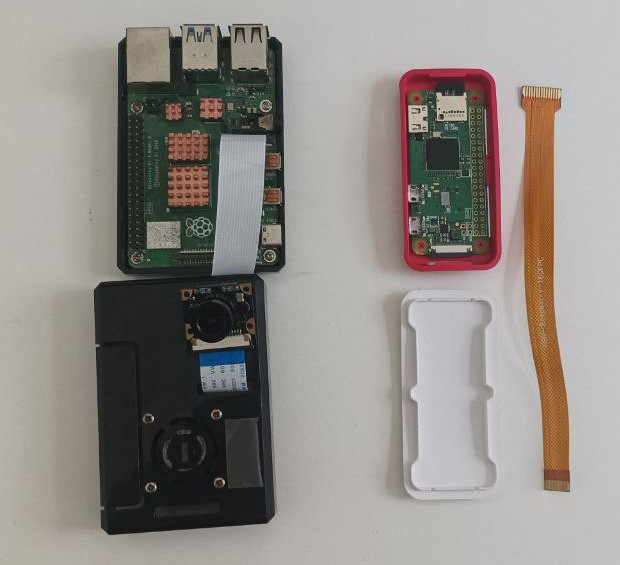
\includegraphics[width=0.6\textwidth]{Cap3_Desenvolvimento/Figures/devices.jpg}
    \caption*{Fonte: autor.}
    \label{fig:devices}
\end{figure}

Apesar de configurações de hardware bem diferentes, os dois dispositivos foram configurados para rodar a mesma versão do sistema operacional Raspberry Pi OS (com kernel 5.10), bem como as mesmas versões do Python (3.7), Picamera (1.13) e OpenCV (3.2). Assim, elimina-se a possibilidade de diferentes versões de software influenciar no desempenho.